\documentclass[12pt]{article}
% \linespread{1.3}
\usepackage{hyperref}
\usepackage{enumitem}
%\usepackage{enumerate}
\usepackage{changepage,lipsum,titlesec, longtable}
\usepackage{cite}
\usepackage{comment, xcolor}
\usepackage[pdftex]{graphicx}
  \graphicspath{{images/}, {images/stat/}}
  \DeclareGraphicsExtensions{.pdf,.jpeg,.png, .jpg}
\usepackage[cmex10]{amsmath}
\usepackage{tikz}
\usepackage{array} 
\usepackage{subfigure} 
\usepackage{geometry}
 \geometry{
 a3paper,landscape
 }
\newcommand{\grey}[1]{\textcolor{black!30}{#1}}
\newcommand{\red}[1]{\textcolor{red!50}{#1}}
\newcommand{\question}[1]{\textcolor{magenta}{\textbf{Question: } {#1}}}
\newcommand{\fref}[1]{Figure~\ref{#1}}
\newcommand{\tref}[1]{Table~\ref{#1}}
\newcommand{\eref}[1]{Equation~\ref{#1}}
\newcommand{\cref}[1]{Chapter~\ref{#1}}
\newcommand{\sref}[1]{Section~\ref{#1}}
\newcommand{\aref}[1]{Appendix~\ref{#1}}

\renewcommand{\labelenumii}{\theenumii}
\renewcommand{\theenumii}{\theenumi.\\arabic{enumii}.}

\oddsidemargin0cm
\topmargin-2cm %I recommend adding these three lines to increase the
\textwidth16.5cm %amount of usable space on the page (and save trees)
\textheight23.5cm

\makeatletter
\renewcommand\paragraph{\@startsection{paragraph}{4}{\z@}%
            {-2.5ex\@plus -1ex \@minus -.25ex}%
            {1.25ex \@plus .25ex}%
            {\normalfont\normalsize\bfseries}}
\makeatother
\setcounter{secnumdepth}{4} % how many sectioning levels to assign numbers to
\setcounter{tocdepth}{4}    % how many sectioning levels to show in ToC

% draw diagram
\usetikzlibrary{shapes.geometric, arrows}
\tikzstyle{anno} = [font=\small]
\tikzstyle{data} = [font=\footnotesize, rectangle, rounded corners, minimum width=3cm, minimum height=1cm,align=left, draw=black, fill=black!30]
\tikzstyle{database} = [font=\footnotesize, rectangle, rounded corners, minimum width=3cm, minimum height=1cm,align=left, draw=black, fill=black!20]
\tikzstyle{query} = [trapezium, trapezium left angle=70, trapezium right angle=110, minimum width=3cm, minimum height=1cm, text centered, draw=black, fill=blue!30]
\tikzstyle{process} = [rectangle, minimum width=3cm, minimum height=1cm, text centered, draw=black, fill=orange!30]
\tikzstyle{spliter} = [diamond, minimum width=2cm, minimum height=1cm, text centered, draw=black, fill=green!30]
\tikzstyle{decision} = [diamond, minimum width=3cm, minimum height=1cm, text centered, draw=black, fill=green!30]
\tikzstyle{arrow} = [thick,->,>=stealth]
\tikzstyle{bi-arrow} = [thick,->,>=stealth]
\begin{document}
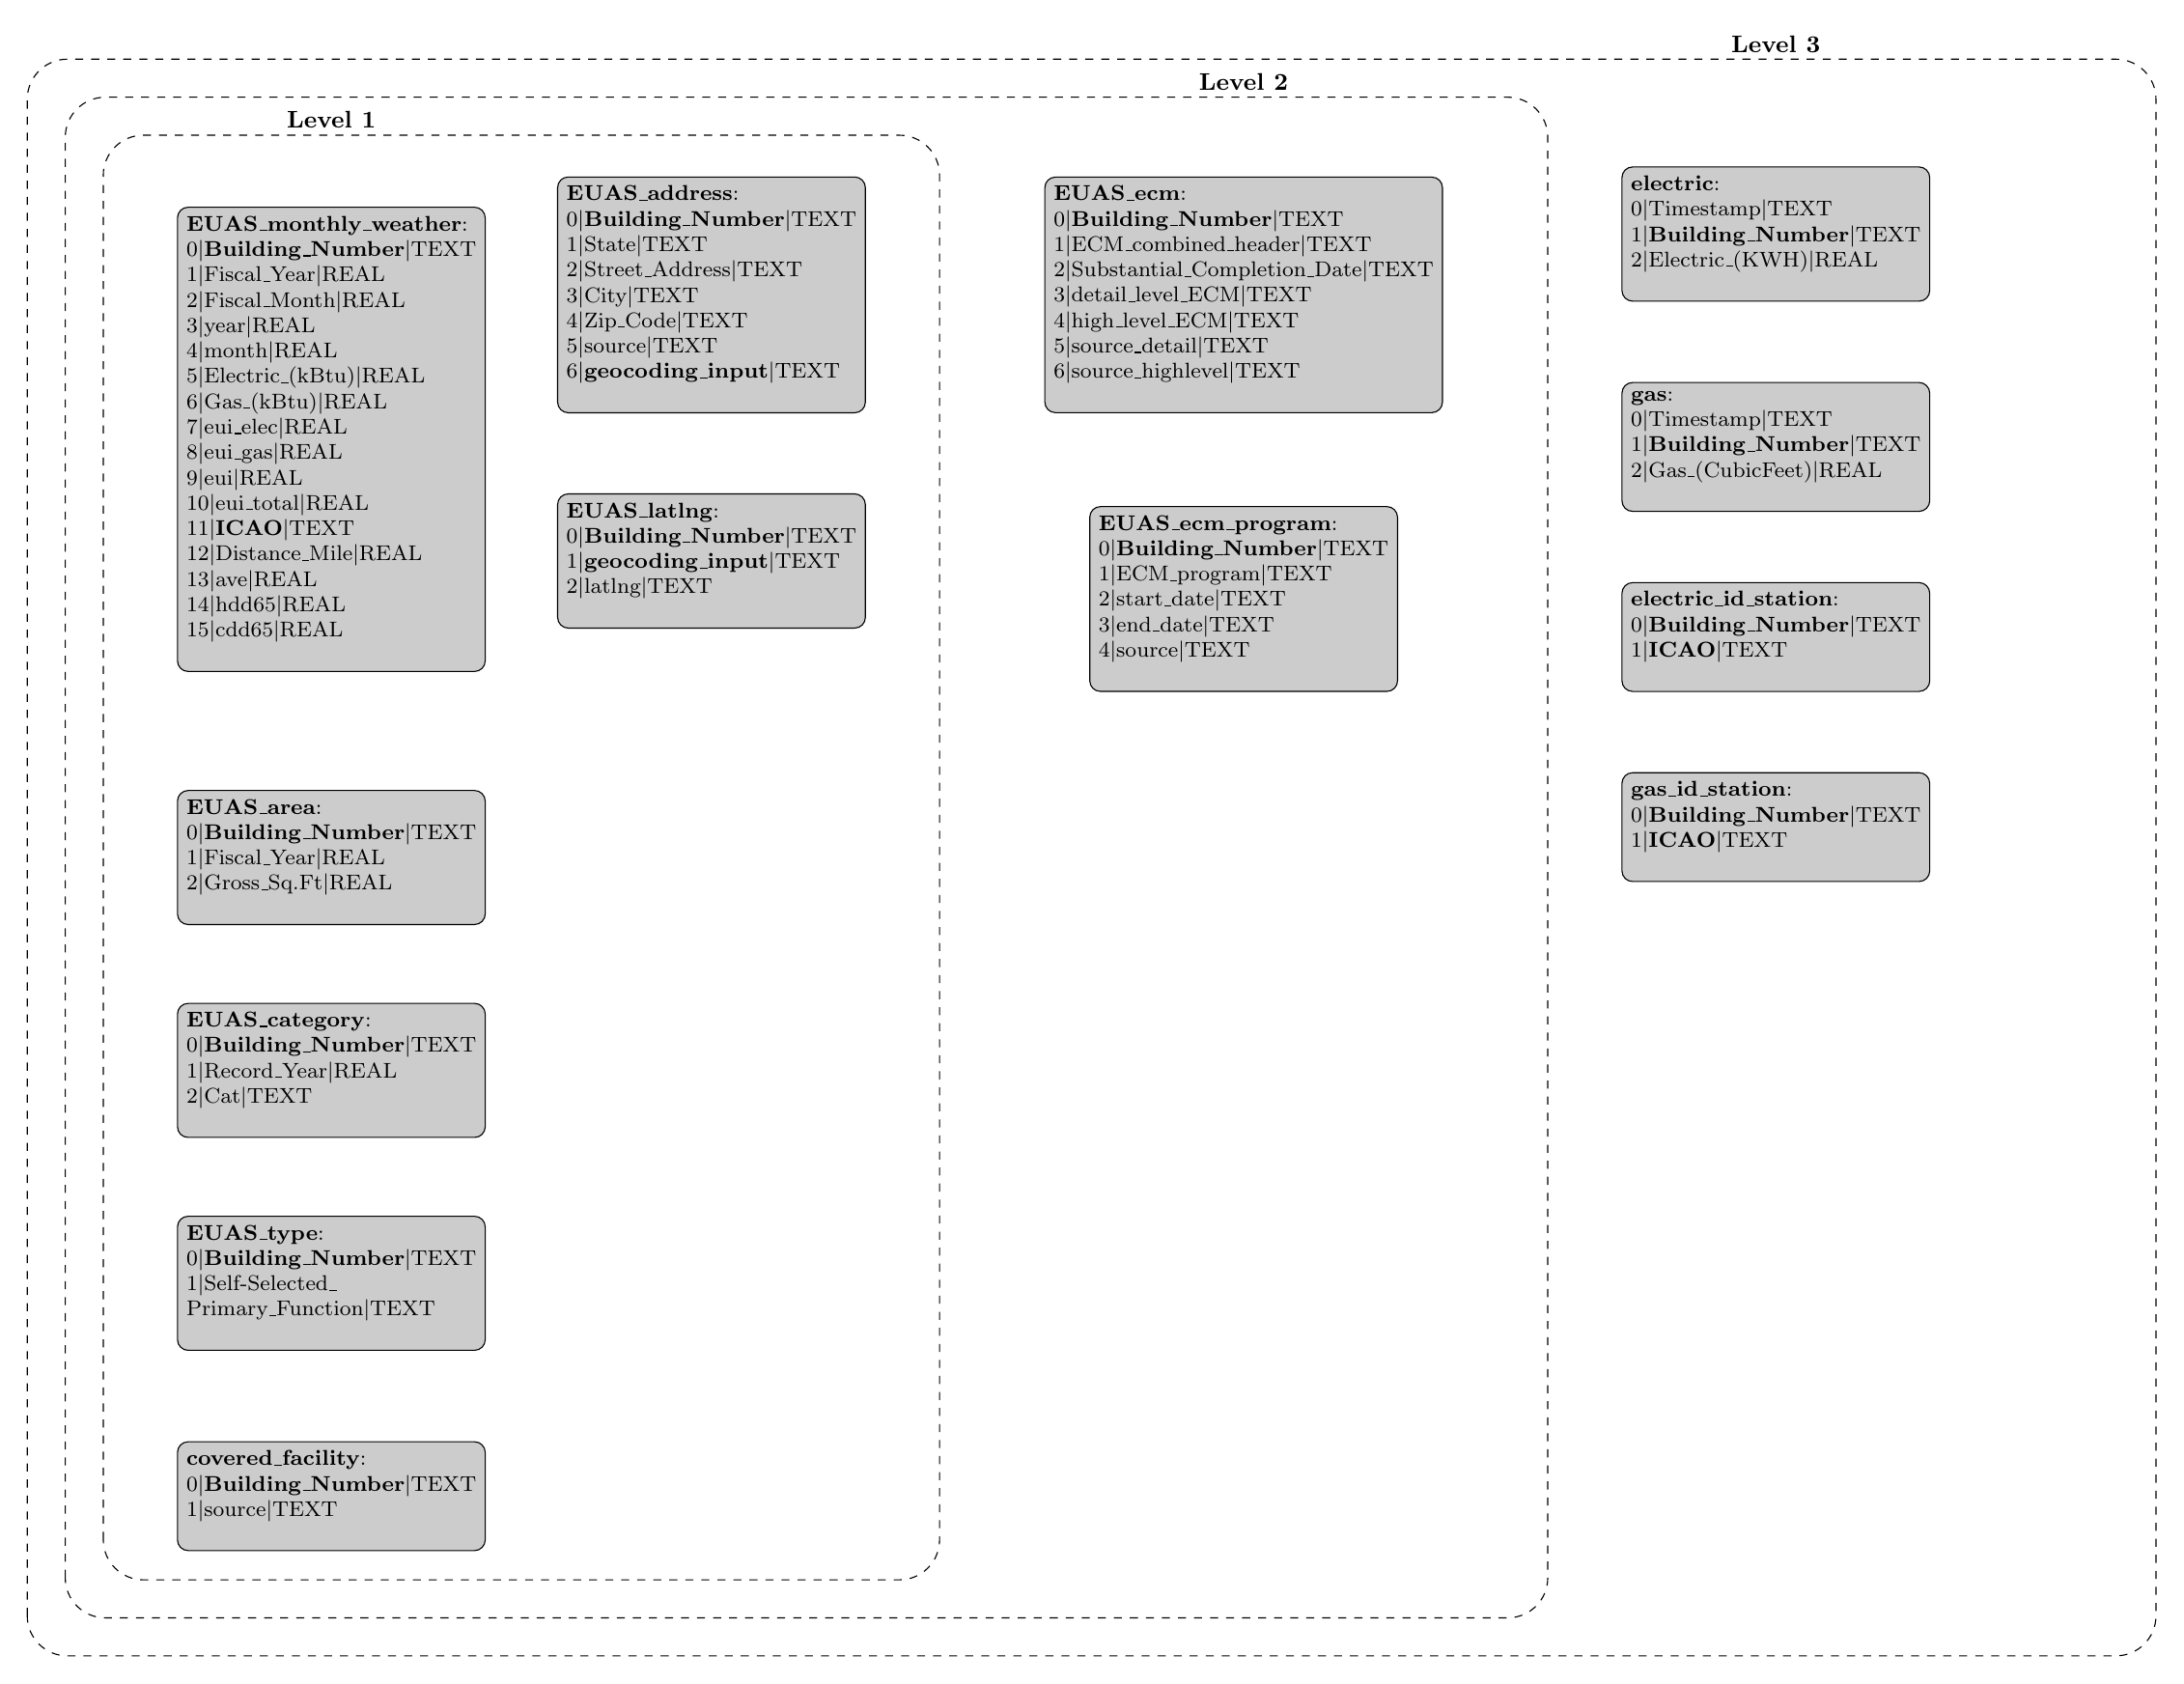
\begin{tikzpicture}
  \node (monthly) [database]{\textbf{EUAS\_monthly\_weather}:\\
0$\lvert$\textbf{\textbf{Building\_Number}}$\lvert$TEXT\\
1$\lvert$Fiscal\_Year$\lvert$REAL\\
2$\lvert$Fiscal\_Month$\lvert$REAL\\
3$\lvert$year$\lvert$REAL\\
4$\lvert$month$\lvert$REAL\\
5$\lvert$Electric\_(kBtu)$\lvert$REAL\\
6$\lvert$Gas\_(kBtu)$\lvert$REAL\\
7$\lvert$eui\_elec$\lvert$REAL\\
8$\lvert$eui\_gas$\lvert$REAL\\
9$\lvert$eui$\lvert$REAL\\
10$\lvert$eui\_total$\lvert$REAL\\
11$\lvert$\textbf{ICAO}$\lvert$TEXT\\
12$\lvert$Distance\_Mile$\lvert$REAL\\
13$\lvert$ave$\lvert$REAL\\
14$\lvert$hdd65$\lvert$REAL\\
15$\lvert$cdd65$\lvert$REAL\\
};
  \node (area) [database, below of=monthly, yshift=-4.5cm]{\textbf{EUAS\_area}:\\
0$\lvert$\textbf{Building\_Number}$\lvert$TEXT\\
1$\lvert$Fiscal\_Year$\lvert$REAL\\
2$\lvert$Gross\_Sq.Ft$\lvert$REAL\\
};
  \node (category) [database, below of=area, yshift=-1.8cm]{\textbf{EUAS\_category}:\\
0$\lvert$\textbf{Building\_Number}$\lvert$TEXT\\
1$\lvert$Record\_Year$\lvert$REAL\\
2$\lvert$Cat$\lvert$TEXT\\
};
  \node (btype) [database, below of=category, yshift=-1.8cm]{\textbf{EUAS\_type}:\\
0$\lvert$\textbf{Building\_Number}$\lvert$TEXT\\
1$\lvert$Self-Selected\_\\Primary\_Function$\lvert$TEXT\\
};
  \node (cover) [database, below of=btype, yshift=-1.8cm]{\textbf{covered\_facility}:\\
0$\lvert$\textbf{Building\_Number}$\lvert$TEXT\\
1$\lvert$source$\lvert$TEXT\\
};
  \node (address) [database, right of=monthly, xshift=4cm, yshift=1.9cm]{\textbf{EUAS\_address}:\\
0$\lvert$\textbf{Building\_Number}$\lvert$TEXT\\
1$\lvert$State$\lvert$TEXT\\
2$\lvert$Street\_Address$\lvert$TEXT\\
3$\lvert$City$\lvert$TEXT\\
4$\lvert$Zip\_Code$\lvert$TEXT\\
5$\lvert$source$\lvert$TEXT\\
6$\lvert$\textbf{geocoding\_input}$\lvert$TEXT\\
};
  \node (latlng) [database, below of=address, yshift=-2.5cm]{\textbf{EUAS\_latlng}:\\
0$\lvert$\textbf{Building\_Number}$\lvert$TEXT\\
1$\lvert$\textbf{geocoding\_input}$\lvert$TEXT\\
2$\lvert$latlng$\lvert$TEXT\\
};
  \node (ecm) [database, right of=address, xshift=6cm]{\textbf{EUAS\_ecm}:\\
0$\lvert$\textbf{Building\_Number}$\lvert$TEXT\\
1$\lvert$ECM\_combined\_header$\lvert$TEXT\\
2$\lvert$Substantial\_Completion\_Date$\lvert$TEXT\\
3$\lvert$detail\_level\_ECM$\lvert$TEXT\\
4$\lvert$high\_level\_ECM$\lvert$TEXT\\
5$\lvert$source\_detail$\lvert$TEXT\\
6$\lvert$source\_highlevel$\lvert$TEXT\\
};
  \node (pro) [database, below of=ecm, yshift=-3cm]{\textbf{EUAS\_ecm\_program}:\\
0$\lvert$\textbf{Building\_Number}$\lvert$TEXT\\
1$\lvert$ECM\_program$\lvert$TEXT\\
2$\lvert$start\_date$\lvert$TEXT\\
3$\lvert$end\_date$\lvert$TEXT\\
4$\lvert$source$\lvert$TEXT\\
};
  \node (ielec) [database, right of=ecm, xshift=6cm, yshift=0.8cm]{\textbf{electric}:\\
0$\lvert$Timestamp$\lvert$TEXT\\
1$\lvert$\textbf{Building\_Number}$\lvert$TEXT\\
2$\lvert$Electric\_(KWH)$\lvert$REAL\\
};
  \node (igas) [database, below of=ielec, yshift=-1.8cm]{\textbf{gas}:\\
0$\lvert$Timestamp$\lvert$TEXT\\
1$\lvert$\textbf{Building\_Number}$\lvert$TEXT\\
2$\lvert$Gas\_(CubicFeet)$\lvert$REAL\\
};
  \node (ielecStation) [database, below of=igas, yshift=-1.5cm]{\textbf{electric\_id\_station}:\\
0$\lvert$\textbf{Building\_Number}$\lvert$TEXT\\
1$\lvert$\textbf{\textbf{ICAO}}$\lvert$TEXT\\
};
  \node (igasStation) [database, below of=ielecStation, yshift=-1.5cm]{\textbf{gas\_id\_station}:\\
0$\lvert$\textbf{Building\_Number}$\lvert$TEXT\\
1$\lvert$\textbf{\textbf{ICAO}}$\lvert$TEXT\\
};
  \node (level1) [anno, above of=monthly, yshift=3.2cm]{\textbf{Level 1}};
  \node (level2) [anno, above of=ecm, yshift=1.8cm]{\textbf{Level 2}};
  \node (level3) [anno, above of=ielec, yshift=1.5cm]{\textbf{Level 3}};
\draw[rounded corners=15pt, dashed] (-3,-15) rectangle (8, 4);
\draw[rounded corners=15pt, dashed] (-3.5,-15.5) rectangle (16, 4.5);
\draw[rounded corners=15pt, dashed] (-4,-16.0) rectangle (24, 5);
%   \node (iarea) [database, below of=iarea]{\textbf{area}:\\
% 0$\lvert$\textbf{Building\_Number}$\lvert$TEXT\\
% 1$\lvert$Gross\_Sq.Ft$\lvert$REAL\\
% };

  % \draw[arrow](PM_table) -- (upload);
  % \draw[arrow](upload) -- (SEED db);
  % \draw[arrow](PM_table) -- (upload2);
  % \draw[arrow](upload2) -- (remote folder);
  % \draw[arrow](remote folder) -- (download);
  % \draw[arrow](download) -- (read);
  % \draw[arrow](read) -- (dataframe);
  % \draw[arrow](dataframe) -| (query);
  % \draw[arrow](query) |- (dataframe);
  % \draw[arrow](dataframe) -- (json);
  % \draw[arrow](json) -- (ext);
  % %\draw[arrow, xshift = -1cm](query) -- (SEED db);
  % %\draw[arrow, xshift = 1cm](SEED db) -- (query);
  % \draw[-latex] (query) to[bend left=10] node [xshift=-1cm]{Street Address} (SEED
  % db); 
  % \draw[-latex] (SEED db) to[bend left=10] node [xshift=2cm,align=center]{buildingsnapshot\_id\\canonical\_building}
  % (query);
\end{tikzpicture}
\end{document}